\chapter{{Application of Bethe-Weizsäcker Mass Formula}}

    \begin{tcolorbox} [colframe=blue!10!black,colback=yellow!29.05!white,arc=1em,fonttitle=\bfseries,title=\textit{Key Objective:}, width = \textwidth]
        $\star$ \textbf{Application of Bethe-Weizsäcker mass formula} $\star$
        \begin{itemize}
            \item Stability of a nucleus against $\alpha$-Decay 
            \item Stability of a nucleus against $\gamma$-Decay 
            \item  Mass parabola 
        \end{itemize}
    \end{tcolorbox}
    
\pagebreak\section{Stability of nucleus against $\alpha$-Decay}
    In the previous chapter we have learnt that Bethe–Weizsäcker mass formula is given by
    
     \begin{equation}
                \begin{split}
                    E_B(A,Z) =a_VA &-a_SA^{2/3} -a_C\frac{Z(Z-1)}{A^{1/3}}\\
                                    & - a_A\frac{(A-2Z)^2}{A} + \delta(A, Z)
                \end{split}
      \end{equation}    
    \par In heavy nuclei, the Coulomb repulsion becomes so strong that we need many additional
neutrons to stabilise the nucleus. It is evident from the nuclear stability line (NZ curve) which tilts
toward the N axis of the curve. It is also apparent if we study the radioactive-decay pattern of the isotopes of heavy nuclei. For
example, if we look at the most
neutron deficient and neutron rich
isotopes of
${}^{89}A$  it is quite apparent. The lighter isotopes prefer to gain stability through
decay due to greater Coulomb
repulsion whereas in heavier
isotopes, it is $\beta$-decay  which we
will learn shortly. Let us look into
the required condition of decay
as per the Bethe–Weizsäcker mass
formula.
$\alpha$-decay  decay of a nucleus, X to the daughter nucleus Y is represented as:


\pagebreak\begin{table}[ht]
        \centering
        \begin{adjustbox}{width=0.8\textwidth}
        \begin{tabular}{|l|c|c|c|}
            \hline
        \textbf{Z} & \textbf{A} & \textbf{Half-Life} & \textbf{Decay mode}\\[0.5cm]\hline
        \textbf{{89} Ac}  & {206} & {22 ms +9-5} &  {$\alpha$}\\
                       {} & {206m} & {33 ms +22-9} & {$\alpha$}\\
                       
                       {} & {207} & {27 ms +22-9} & {$\alpha$}\\
                       
                       {} & {208} & {95 ms +24-16} & {$\alpha$ $\approx99$ $\%$,$\epsilon$$\approx1$$\%$}\\[0.5em]
                       
                       {} & {208m} & {25 ms +9-5} & {$\alpha$ $\approx90$ $\%$,$\epsilon$ $\approx10$ $\%$}\\[0.5em]
                       
                       {} & {209} & {0.10 s 5} & {$\alpha\approx99\%,\epsilon \approx1\%$}\\[0.5em]
                       
                       {} & {210} & {0.35 s 5} & {$\alpha\approx91\%,~\epsilon \approx9$\%}\\[0.5em]
                       
                       {} & {211} & {0.21 s 3} & {$\alpha$}\\
                       
                       {} & {212} & {0.93 s 5} & {$\alpha\approx57\%,~\epsilon \approx43\%$ }\\[0.5em]
                       
                       {} & {227} & {21.772 y 3} & {$\beta\approx$- 98.62$\%$, $\alpha\approx$ 1.38$\%$}\\[0.5em]
                  
                       {} & {228} & {6.15 h 2} & {$\beta$-}\\
                       
                       {} & {229} & {62.7 m 5} & {$\beta$-}\\
                       
                       {} & {230} & {122 s 3} & {$\beta$-,~$\beta-\approx~ 1.2*10^-6\% $}\\[0.5em]
                       
                       {} & {231} & {7.5 3 1} & {$\beta$-}\\
                       
                       {} & {232} & {119 s 5} & {$\beta$-}\\
                       
                       {} & {233} & {145 s 10} & {$\beta$-}\\
                       
                       {} & {234} & {44 s 7} & {$\beta$-}\\
                       
                       {} & {235} & {60 s 4} & {$\beta$-}\\
                       
                       \hline
                  
        \end{tabular}            
        \end{adjustbox}

 \label{tab:table_decaymode}
\caption{Half-life and decay mode of nine most lightest and heaviest isotopes of Actinum(Ac).}
 \end{table}
    \begin{equation}
   {}^{A}_{Z}X  \longrightarrow {}^{A-4}_{Z-2}Y +{}^{4}_{2}He(\alpha)
     \end{equation}

We have learned to calculate the disintegration energy Q as follows,
\begin{equation}
Q_\alpha=M(A,Z)- M(A-4,Z-2)-M_\alpha
\end{equation}

Since total numbers of neutrons and protons are constants, if we substitute the M’s according
to the binding energy formula $E_B=ZM_H+NM_n-M(A, Z)$
it gives us,
\begin{equation}
Q_\alpha=E_B(A-4,Z-2)+E_B(\alpha)-E_B(A,Z)
\end{equation}   
   
 Using the Bethe–Weizsäcker mass formula, we can rewrite the above equation
\begin{multline}
Q_\alpha=a_V(A-4)-a_S(A-4)^{2/3}-a_C\frac{(Z-2)}{(A-4)^{1/3}}-a_A\frac{(A-2Z)^2}{(A-4)}\\
~-a_VA+a_SA^{2/3}+\frac{Z^2}{A^{1/2}}+a_A\frac{(A-2Z)^2}{A}+E_B(\alpha)
\end{multline} 

 
\par We have replaced Z(Z-1) as $Z^2$.  The total binding energy of $\alpha$ particle is 28.3 MeV. Thus,
  \begin{equation}
  Q_\alpha=28.34a_V+a_S\frac{8/3}{A^{-1/3}}+a_C\frac{4Z}{A^{1/2}}(1-\frac{Z}{3A})-a_A\frac{4(A-2Z)^2}{A(A-4)}
  \end{equation}

If we replace the proportionality constants (a’s) with their estimated values, the $Q_\alpha>0$  (condition to occur $\alpha$-decay) for $A>160$ which is close to the experimental value.


   
\pagebreak\section{{Stability of nucleus against $\beta$-Decay}}
 
\subsection{The Mass Parabola and stability:}
   The Bethe–Weizsäcker mass formula is a function of A and Z. Therefore, it gives us the opportunity to study
the behaviour of M(A, Z) as a function of Z. It will
help us find out the most stable Z value for nuclei
with a fixed A (i.e. isobar: nuclei with same mass
number A). We rewrite the mass formula as a
function of Z as,
\begin{equation}
\begin{split}
     M(A, Z)=K_1+K_2Z+K_3Z^2{\pm}\delta
\\ \textrm where,
\\\textrm K1=A(M_n-a_V+a_A+a_S^{-1/3}),
 \\\textrm K2=-[4a_A+(M_n-M_H)],
  \\ \textrm K3=(4\frac{a_A}{A}+\frac{a_C}{A^{1/3}}).
\end{split}
\end{equation}
 
\par Since $\delta$ is independent of A, we may neglect it.
The variation of M(A, Z) takes the form of a parabola for a given A. For a particular Z value, M(A,Z) reaches the minimum of the curve and it corresponds to the most stable nucleus for that A.The adjoining figure is showing a representative mass parabola for A=135 (Source: MIT OCW,
22.101 Applied Nuclear Physics, Fall 2006). The most stable nucleus $(Z_A)$  for this mass number is ${}^{56}B $.

     We can obviously calculate it as 
\begin{align}
\frac{\delta M(A,Z)}{\delta Z}=0=K_2+2k_3Z_A\\
\textrm{So,}
~~Z_A= -\frac{K_2}{2K_3}=\frac{(M_n-M_H+4a_A)A}{2(a_cA^2/3+4a_A)}
\end{align}
     
If we substitute $Z_A$ in the expression of M(A,Z), we get 
\begin{equation}
 \begin{split}
 M(A,Z_A)=K_1+K_2&(-K_2/2K_3)+K_3\frac{K_2^2}{4K_3^2}=K_1-\frac{K_2^2}{4k_3}\\
\textrm{So,}~~M(A,Z_A)-M(A,&~Z_A)=\frac{K_2^2}{4K_3^2}+K_2Z+K_3Z^2\\&=K_3(Z^2-2Z_AZ+Z_A^2)\\
\therefore M(A,Z)-&M(A,Z_A)=K_3(Z-Z_A)^2 
\end{split}  
\end{equation} 

   
It shows that at $Z=Z_A$ , a mass parabola reaches its minima for a given A value. It gives an approximate value of the transition energies in $\beta$-decay reactions. The usefulness of the above exercise can be appreciated in many ways. Let us substitute the values of $M_n, M_H, a_C $ and $a_A $ and we get
  \begin{equation}
  Z_A=\frac{A}{1.98+0.015A^{2/3}}
   \end{equation}
   
  For a given A, the above expression provides a fairly accurate estimate of the corresponding $Z_A$.For example, if we replace A with 63, the corresponding $Z_A = 28.4$. Experimentally the most stable nucleus for A=63 is Cu (Z=29).The expression for also gives us an idea of the effect of Coulomb force. If we neglect the asymmetry term is that expression, it becomes,
  \begin{equation}
  Z_A=\frac{(M_n-M_H)A}{2a_CA^{2/3}}=\approx-.9A^{1/3}
      \end{equation}

For Z=18, A is 8000 which is unrealistic! It clearly demonstrates that the Coulomb force is really responsible for observation of the deviation of the line of stability from the N=Z line.

\begin{wrapfigure}{l}{0.5\textwidth}
         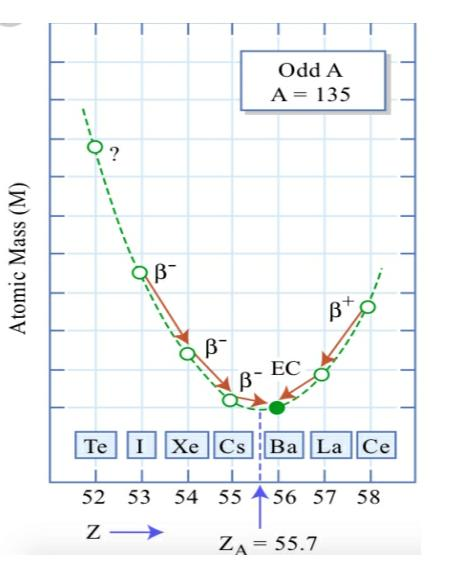
\includegraphics[width =0.48\textwidth]{04/ZVM_plot.jpg}
         \caption{Z vs M Plot(for odd A)}
         \label{fig:plot_ZvsM}
\end{wrapfigure}
     
\subsection{Stability of a nucleus against $\beta$-decay:}   The obvious question might have come to your mind “what will happen to the other nuclei of the mass parabola away from $Z_A $ ?”. Actually this question answers one of the most important aspects of the mass parabola: The origin of $\beta$ instability or the origin of $\beta$-decay. The only way to reach the minima of the mass parabola without changing A value is to undergo $\beta$-decay. The nuclei away from with $Z > Z_A$ undergo $\beta^-$ decay. It is represented as
     \begin{equation}
        {}^{A}_{Z}X  \longrightarrow {}^{A}_{Z+1}Y  + \beta^-+\gamma 
      \end{equation}
      
\begin{wrapfigure}{r}{0.5\textwidth}
    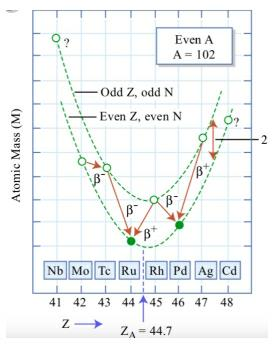
\includegraphics[width=0.48\textwidth]{04/ZVA_plot.jpg}
    \caption{Z vs M plot (for even A)}
    \label{fig:plot_ZvsM2}
\end{wrapfigure}

\par $\gamma$ is a nearly massless, chargeless fermion and $\gamma$ is the anti-neutrino. We will discuss it in due course of time. In the above mass parabola picture, the nuclei Te, I, Xe, and Cs are going through successive
$\beta^-{}$ decay to increase their Z value until ${}^{135}B $ is reached.

Similarly, nuclei with $ Z > Z_A $ undergo decay to decrease their Z values to reach the minima. A typical $\beta^+{}$ decay to reach the minima.
\begin{equation}
  {}^{A}_{Z}X \longrightarrow {}^{A}_{Z-1}Y  + \beta^+ + \gamma
\end{equation}

 In the above figure, Ce and La undergo repeated $\beta^+$ decay to reach the minima.
 
 It is interesting to note that in case of even-A nuclei,there are two possibilities; a) both N and Z are odd (odd-odd) and b) both N and Z are even (even-even).In the first -$\delta$ case and for the later case, it is +$\delta$ .Therefore, we get two mass parabolas instead of one with their minima shifted by . The adjoining figure \ref{fig:plot_ZvsM2}
({\textit{\textbf{Source:} MIT OCW, 22.101 Applied Nuclear Physics, Fall 2006}})
clearly demonstrates this fact.



One thing should be mentioned that few nuclei undergo double $\beta$-decay. In ordinary double $\beta$-decay, two neutrons are converted into protons inside the nucleus. Two electrons and two electron type $\gamma$ are emitted. However, only very few nuclei (14
nuclei between ${}^{48}Ca $ and ${}^{238}U $) have shown double $\beta$-decay. It will only be possible, if the final nucleus has greater binding energy than the original nucleus. One example is ${}^{76}Ge $ .The most stable for A=76 isobars is ${}^{76}Se $ . The ${}^{76}Ge $ should undergo a $\beta^-$-decay  and form $^{76}As$ which in turn perform another  $\beta^-$-decay to reach the minima at ${}^{76}Se $ . However, $^{76}As$ has a smaller binding energy than ${}^{76}Ge $ which prevents the single $\beta^-$-decay. The ${}^{76}Se $ , on the other hand, has larger binding energy which allows the ${}^{76}Ge $ to go through double $\beta$-decay. Conceptually it is possible to have neutrinoless double $\beta^-$-decay where only electrons would be emitted. However, experimentally it is yet to be observed.